\section{VI. Các biểu đồ khảo sát}

% 1
\begin{frame}
    \frametitle{Mức độ chơi game thường xuyên:}
    
    \begin{figure}[H]
        \centering
        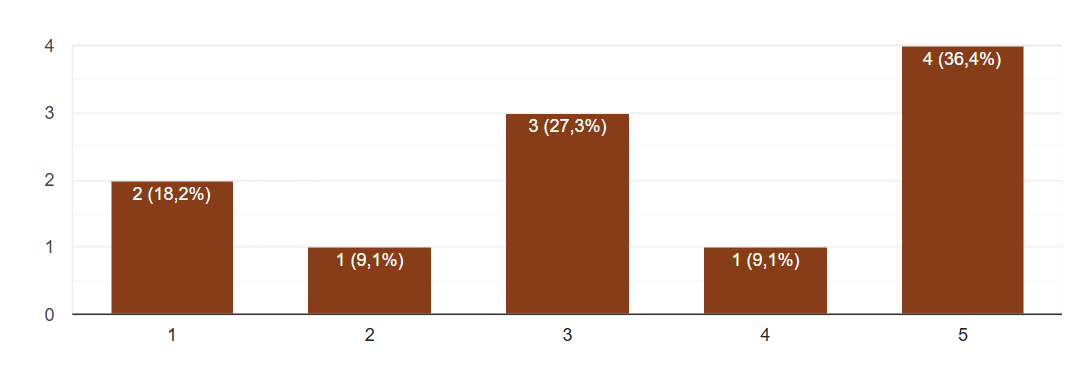
\includegraphics[width=1\linewidth]{bieu-do/muc-do-choi-game.png}
    \end{figure}
\end{frame}

% 2
\begin{frame}
    \frametitle{Chất lượng đồ họa tổng quan:}
    \begin{figure}[H]
        \centering
        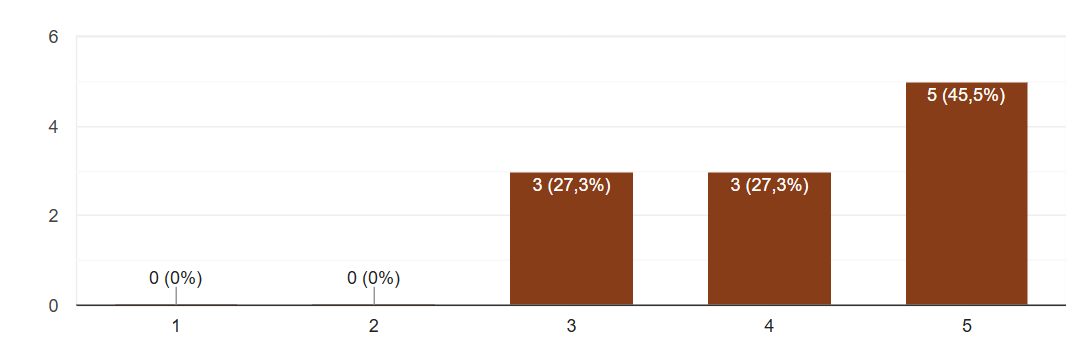
\includegraphics[width=1\linewidth]{bieu-do/chat-luong-do-hoa-tong-quan.png}
    \end{figure}
\end{frame}

% 3
\begin{frame}
    \frametitle{Chất lượng đồ họa nhân vật 3D:}
    \begin{figure}[H]
        \centering
        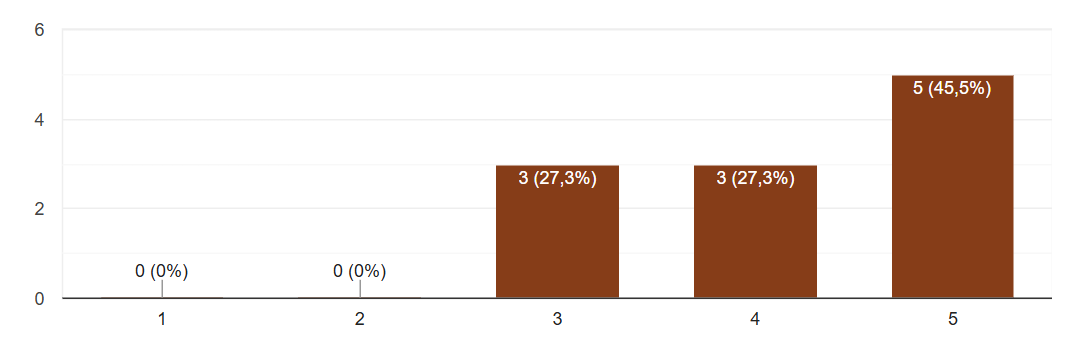
\includegraphics[width=1\linewidth]{bieu-do/do-hoa-nhan-vat.png}
    \end{figure}
\end{frame}

% 4
\begin{frame}
    \frametitle{Chất lượng đồ họa cảnh quan, môi trường:}
    \begin{figure}[H]
        \centering
        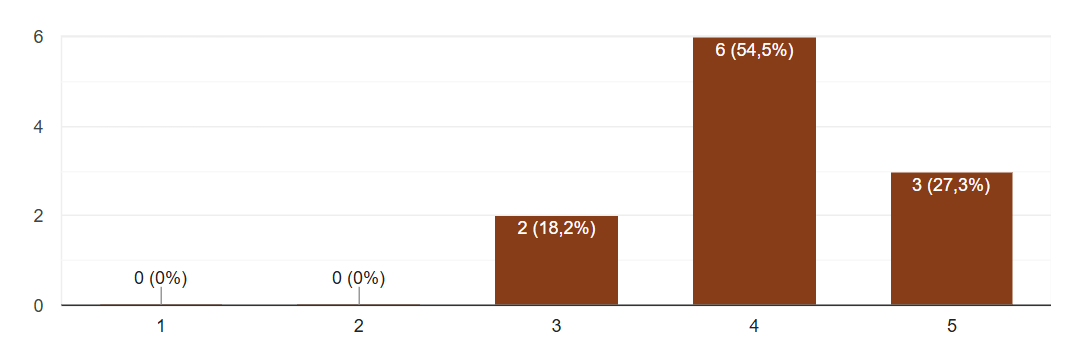
\includegraphics[width=1\linewidth]{bieu-do/canh-quan-moi-truong.png}
    \end{figure}
\end{frame}

% 5
\begin{frame}
    \frametitle{Chất lượng của các thẻ bài, item liên quan đến board game:}
    \begin{figure}[H]
        \centering
        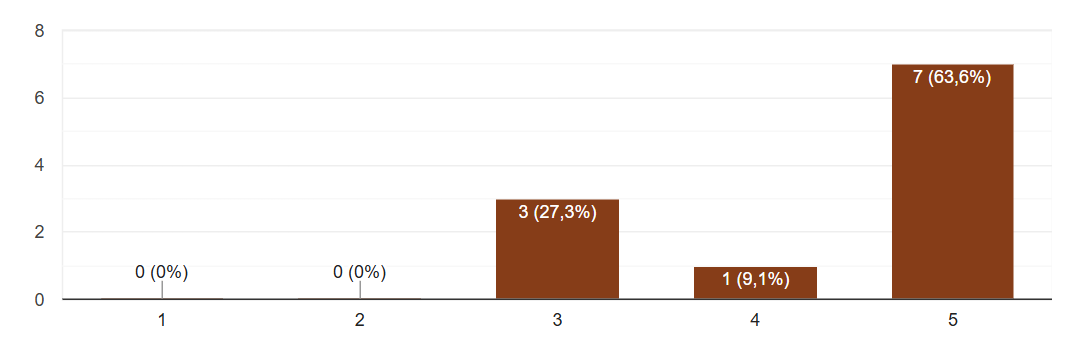
\includegraphics[width=1\linewidth]{bieu-do/the-bai-chat-luong.png}
    \end{figure}
\end{frame}


% 6
\begin{frame}
    \frametitle{Giao diện người dùng (UI) phù hợp:}
    \begin{figure}[H]
        \centering
        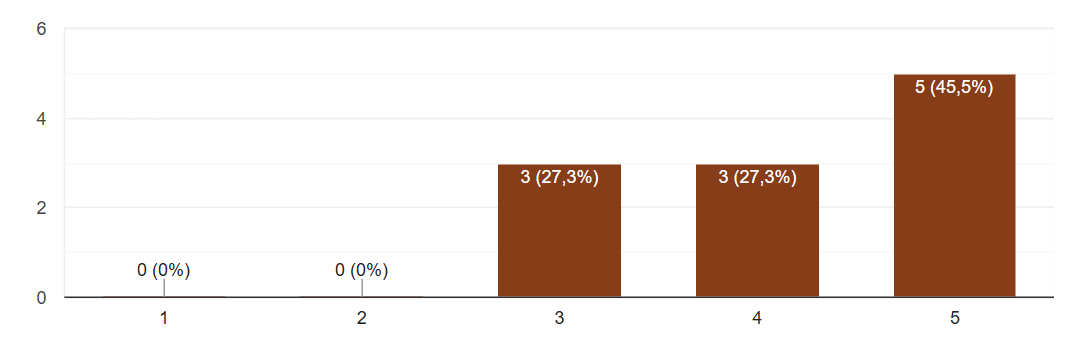
\includegraphics[width=1\linewidth]{bieu-do/ui-phu-hop.png}
    \end{figure}
\end{frame}

% 7
\begin{frame}
    \frametitle{Hiệu ứng âm thanh và nhạc nền phù hợp:}
    \begin{figure}[H]
        \centering
        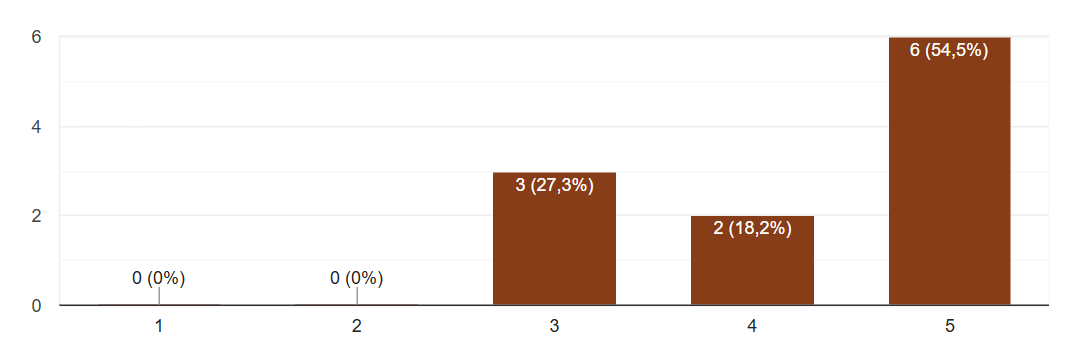
\includegraphics[width=1\linewidth]{bieu-do/am-thanh.png}
    \end{figure}
\end{frame}

% 8
\begin{frame}
    \frametitle{Đánh giá độ mượt mà điều khiển của nhân vật với các hành động chung (di chuyển, ngồi, nhảy, emote,..):}
    \begin{figure}[H]
        \centering
        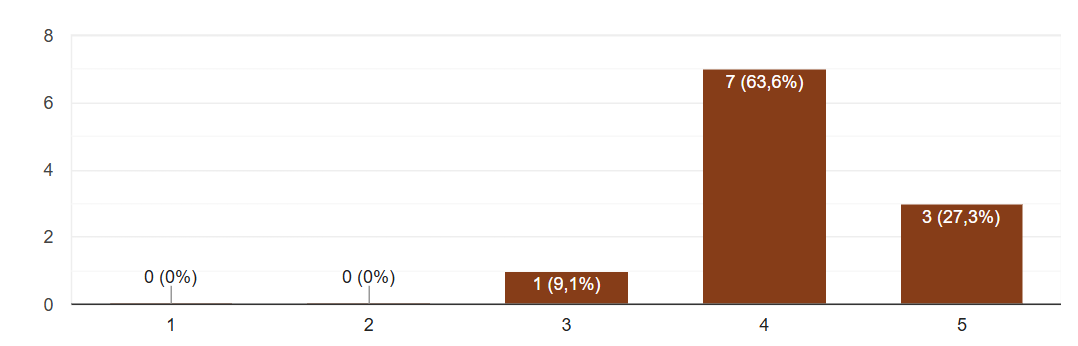
\includegraphics[width=1\linewidth]{bieu-do/character-muot-ma.png}
    \end{figure}
\end{frame}

% 9
\begin{frame}
    \frametitle{Độ mượt mà và góc máy của Camera :}
    \begin{figure}[H]
        \centering
        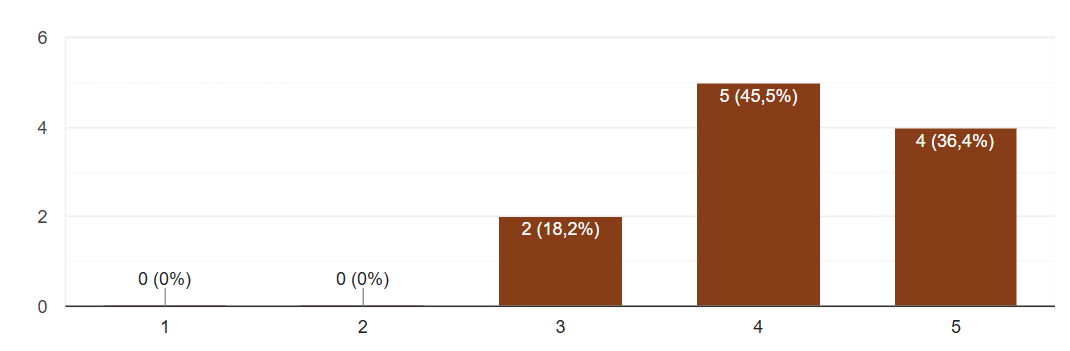
\includegraphics[width=1\linewidth]{bieu-do/camera-muot-ma.png}
    \end{figure}
\end{frame}



%% class bieu-do

% 10
\begin{frame}
    \frametitle{Độ mượt mà khi điều khiển, chọn các thành phần UI:}
    \begin{figure}[H]
        \centering
        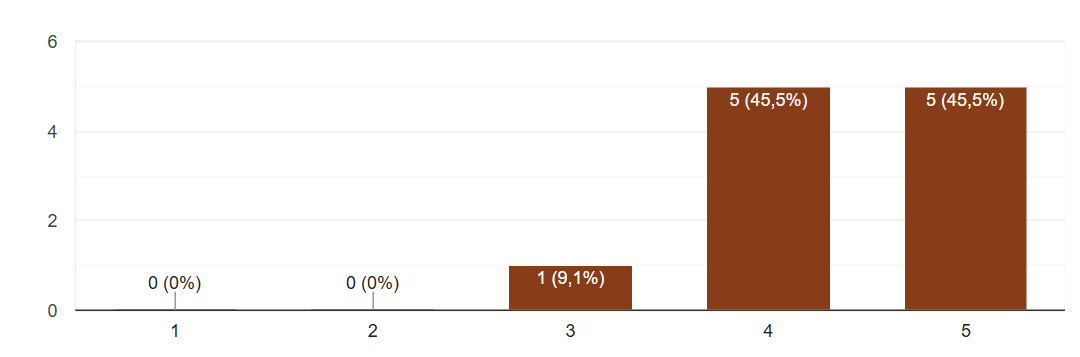
\includegraphics[width=1\linewidth]{bieu-do/ui-muot-ma.png}
    \end{figure}
\end{frame}

% 11
\begin{frame}
    \frametitle{Độ mượt mà của điều khiển các thẻ bài (chọn bài, bỏ bài, chọn chỗ đặt, chọn người chơi,...):}
    \begin{figure}[H]
        \centering
        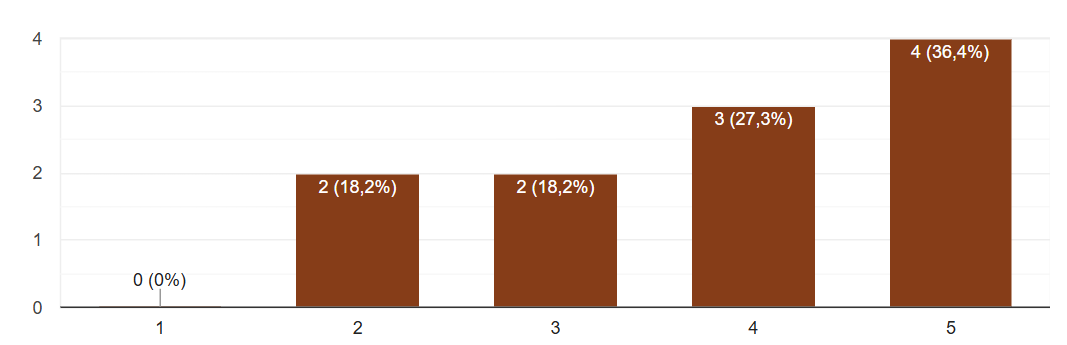
\includegraphics[width=1\linewidth]{bieu-do/control-the-bai-muot-ma.png}
    \end{figure}
\end{frame}

% 12
\begin{frame}
    \frametitle{Độ mượt mà về hiệu năng game, hiện tượng tụt FPS:}
    \begin{figure}[H]
        \centering
        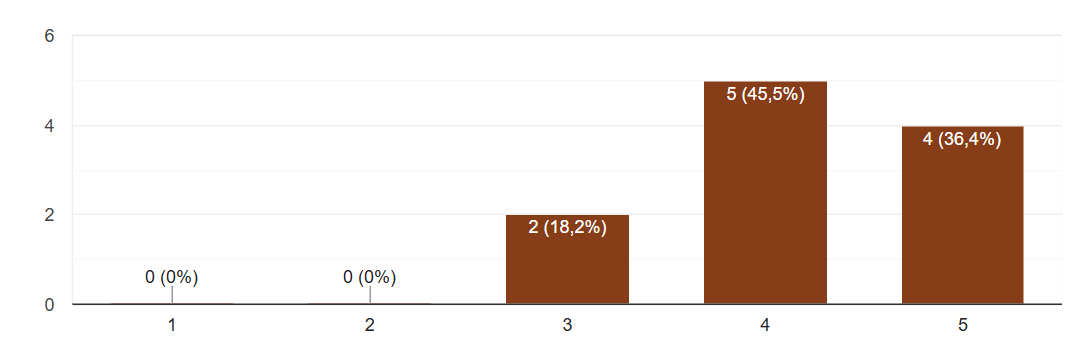
\includegraphics[width=1\linewidth]{bieu-do/fps-muot-ma.png}
    \end{figure}
\end{frame}

% 13
\begin{frame}
    \frametitle{Độ mượt mà về Networking, hiện tượng người chơi teleport:}
    \begin{figure}[H]
        \centering
        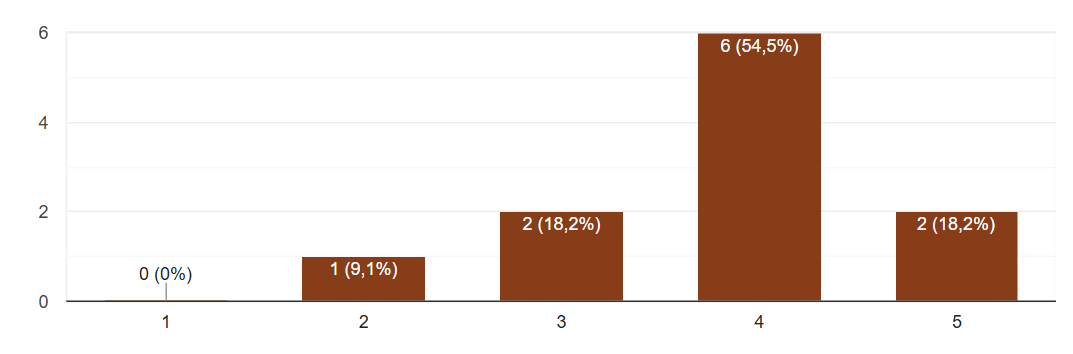
\includegraphics[width=1\linewidth]{bieu-do/network-muot.png}
    \end{figure}
\end{frame}

% 14
\begin{frame}
    \frametitle{Độ mượt mà của kênh chat (voice chat, text chat):}
    \begin{figure}[H]
        \centering
        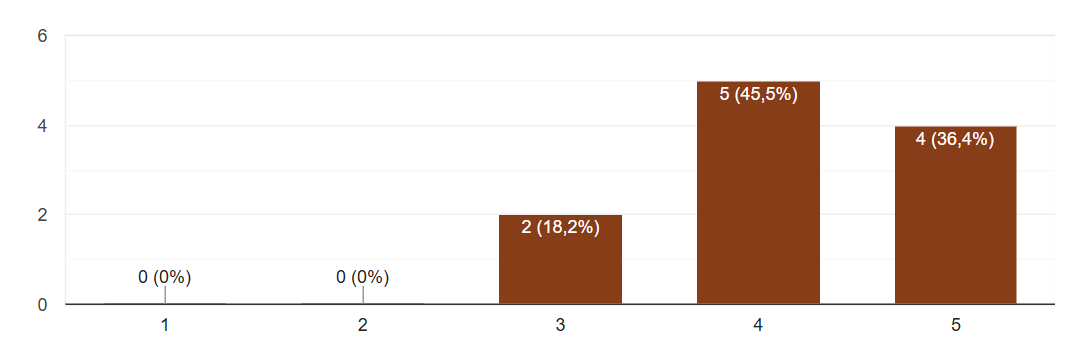
\includegraphics[width=1\linewidth]{bieu-do/chat-muot-ma.png}
    \end{figure}
\end{frame}

% 15
\begin{frame}
    \frametitle{Lối chơi, độ hấp dẫn của board game - classic mode:}
    \begin{figure}[H]
        \centering
        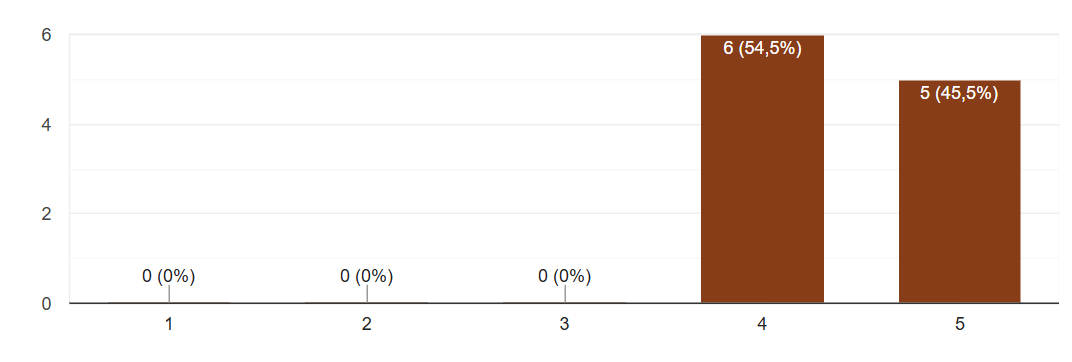
\includegraphics[width=1\linewidth]{bieu-do/classic-hap-dan.png}
    \end{figure}
\end{frame}

% 16
\begin{frame}
    \frametitle{Lối chơi, độ hấp dẫn của board game - day \& night mode:}
    \begin{figure}[H]
        \centering
        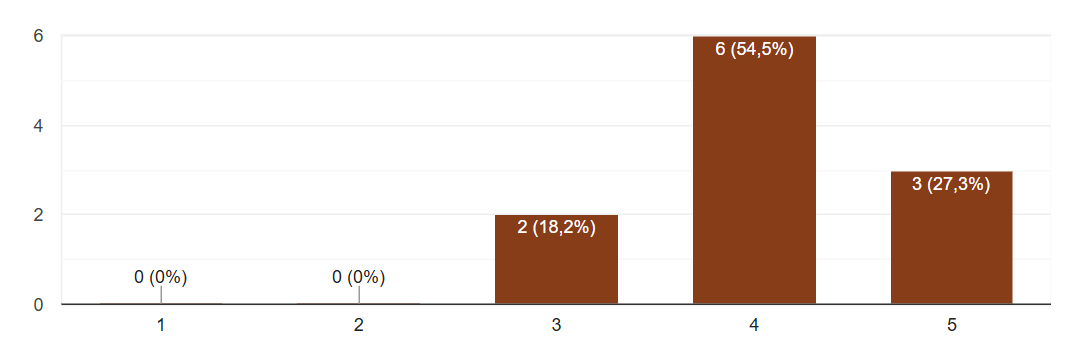
\includegraphics[width=1\linewidth]{bieu-do/day-nigh-hap-dan.png}
    \end{figure}
\end{frame}

% 17
\begin{frame}
    \frametitle{Luật chơi dễ nắm bắt, thông tin chi tiết của các bài qua tooltip, gameplay info:}
    \begin{figure}[H]
        \centering
        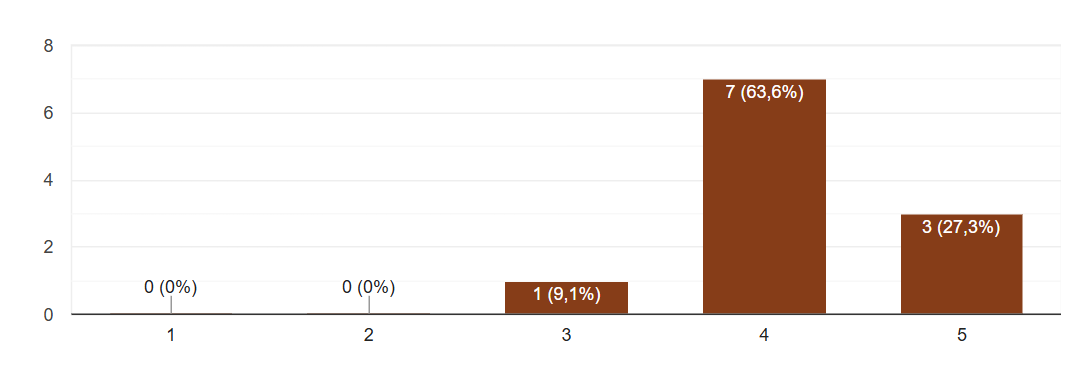
\includegraphics[width=1\linewidth]{bieu-do/luat-choi-de-nam-bat.png}
    \end{figure}
\end{frame}